\documentclass[11pt, oneside]{article}
\usepackage[margin=1in,letterpaper]{geometry}
\usepackage{times}
\usepackage{graphicx}
\usepackage{amssymb,amsmath,mathtools}
\usepackage{array}
\usepackage{longtable}
\usepackage{color}
\usepackage[T1]{fontenc}
\usepackage{sectsty}
\usepackage{tikz}
\usetikzlibrary{decorations.pathmorphing,decorations.markings,calc,patterns,arrows.meta,shapes.geometric}
\sectionfont{\fontsize{12}{12}\selectfont}
\subsectionfont{\fontsize{11}{11}\selectfont}
\subsubsectionfont{\normalsize\itshape\mdseries}

\renewcommand\labelitemi{{\boldmath$\cdot$}}
% NOTE: dots at every level; the handwritten dashes are set explicitly with \item[--].
\renewcommand\labelitemii{\labelitemi}
\renewcommand\labelitemiii{\labelitemi}
\renewcommand\labelitemiv{\labelitemi}

%%%%%%%%%%%%%%%%%%%%%%%%%%%%%%%%%%%%%
% Notation: symbols follow ../variables_master.tex. The handwriting follows Ulaby & Long (2014), Ch. 8, for the
% atmosphere. Instructor decisions (2026-09-29, master table D85--D99): renamed (resolved): water-vapor density and
% scale height rho_v, rho_v0, H_v -> rho_vap, rho_vap,0, H_vap (D85); sea-level air density rho_0 -> rho_air,0 (D86);
% moist lapse rate a_w = f(T,P) -> a_moist(T,P) (D91, D92); gas constant R -> R_gas (D93); molecular energies
% U, U_e, U_v, U_r -> script E, E_e, E_v, E_r, as in U&L Eq. 8.9 (D95); rotation and vibration angular frequencies
% omega -> omega_rot, omega_vib (D96); rotational quantum number l -> J, as in Liou (D98); vibrational quantum
% number n_v -> n_vib (D99). Kept (approved): rho_air (D86), pressure P (D87), subscript 0 = sea level (D88), c_p
% (D89), lapse rates a, a_d (D90), scale heights H_p, H_rho (D94), Planck h and hbar (D97, formerly F4).
% Not triggered in this lecture (no optical depth, phase function, mu = cos theta, Stefan--Boltzmann constant, or
% photon energy E appears): F2, F3, F6, F8, F11.
% Subscripts: descriptive (word) subscripts are upright, as in Ulaby & Long and Lecture 9. The conventional c_p is
% italic, and H_p (pressure) follows it; H_rho is the density scale height. Chemical symbols are upright.
% Main reference checks: Ulaby & Long (2014), Sec. 8-1 and 8-2.1 (pp. 326-329), Eqs. 8.1-8.9, Figs. 8-2, 8-3;
% Liou (2002), Sec. 1.3.1.2 (pp. 16-21), Eqs. 1.3.5-1.3.9, Fig. 1.10; Sec. 3.1.1 (pp. 65-67), Fig. 3.1.
%%%%%%%%%%%%%%%%%%%%%%%%%%%%%%%%%%%%%

% NOTE: the handwriting has no title; page L1 reads "12.421/12.621 Lecture 10". The title is that of the matching
% slide deck, princRS_lecture10.key ("Interaction of EM radiation with atmospheres"), which also matches the
% handwritten heading on page L2 ("Interaction of EM radiation and atmospheres"); the Lecture 11 deck ("Atmospheric
% absorption and emission Part 2") continues this lecture's last section.
\title{12.421/12.621 Lecture 10: Interaction of EM Radiation with Atmospheres}
\author{Brent Minchew}
\date{}

\setlength{\emergencystretch}{1.5em}
\renewcommand{\topfraction}{0.85}
\renewcommand{\textfraction}{0.1}
\renewcommand{\floatpagefraction}{0.75}
\begin{document}
\maketitle

\noindent\underline{\textbf{Topics covered}}
\begin{itemize}
	\item Review of Earth's atmosphere structure
	\item Brief discussion of temperature lapse rate and pressure and density profiles
	\item Absorption and emission by gases in the atmosphere
\end{itemize}

%%%%%%%%%%%%%%%%%%%%%%%%%%%%%%%%%%%%%
\section{Interaction of EM radiation and atmospheres}
\label{s:intro}

\begin{itemize}
	\item Virtually all remote sensing applications need to contend with atmosphere, whether the atmosphere is signal or noise.
	\item As we saw, the transparency of the atmosphere varies with EM frequency from virtually opaque to virtually transparent in a way that may appear at first glance to be quasi-random.
	\item To understand how the atmosphere can be observed with remote sensing and can influence terrestrial observations, we start with basic definitions of the atmosphere.
\end{itemize}

%%%%%%%%%%%%%%%%%%%%%%%%%%%%%%%%%%%%%
\section{Standard atmosphere of Earth}
\label{s:std}

\begin{itemize}
	% NOTE: kept as handwritten. Liou (2002, p. 66) and U&L (2014, p. 326) divide the thermal profile into four layers
	% (troposphere, stratosphere, mesosphere, thermosphere), with the exosphere above the thermosphere (Liou p. 67);
	% the handwriting counts the exosphere as the fifth.
	\item Earth's atmosphere is made up of 5 primary layers. Layer boundaries are defined by changes in thermal lapse rate. From top to bottom, the layers are
	\begin{itemize}
		\item Exosphere
		\begin{itemize}
			% NOTE: AMSL = above mean sea level. Outside source (not in Liou or U&L): the exobase is commonly placed at
			% ~500-1000 km depending on solar activity, and ~700 km to ~10^4 km is the usual quoted range.
			\item[--] Altitude range ${\sim}700$~km (AMSL) -- ${\sim}10^4$~km
			\item[--] Extremely low density
			% NOTE: the handwritten "also known as thermopause" is attached to "exobase" by a curved arrow; set in
			% parentheses.
			\item[--] bottom is defined by ``exobase'' (also known as thermopause) ${\sim}$ orbital altitude of many Earth-observing satellites
			\item[--] low density $+$ high altitude $\rightarrow$ negligible for most RS applications
		\end{itemize}
		\item Thermosphere
		\begin{itemize}
			\item[--] Altitude range ${\sim}80$~km -- ${\sim}700$~km
			\item[--] low density (many satellites and ISS orbit here)
			% NOTE: handwritten reads "from ~190 K to ~330 K (in International Standard Atmosphere"; kept, with the
			% scope added: 190-330 K is the range from the mesopause to 120 km, the top of U&L 2014, Fig. 8-3 (p. 326;
			% the curve reaches the 333 K edge of the plot at 120 km). Higher in the thermosphere, temperatures range
			% from 500 K to as high as 2000 K, depending on the level of solar activity (Liou 2002, p. 67), so 330 K is
			% not the temperature at the top of the thermosphere (~700 km). (U&L call the thermosphere curve "modeled", p. 327;
			% ISA itself is formally defined only to 80 km, so the 330 K is tied to the U&L profile, not to ISA.)
			\item[--] temperature increases with elevation (temperature inversion) from ${\approx}190$~K to ${\approx}330$~K (in International Standard Atmosphere; 330~K is reached at 120~km altitude, where the standard profile of Ulaby and Long (2014), Fig.~8-3, ends; higher up, temperatures reach 500--2000~K, depending on solar activity)
			\item[--] top is defined by exobase (a.k.a.\ thermopause)
			\item[--] bottom defined by mesopause
			% NOTE: kept as handwritten. Outside source: the ionosphere spans ~60 km (D region, in the mesosphere) to
			% ~1000 km, with its peak electron density (F2 layer) at ~250-400 km, within the thermosphere.
			\item[--] Importantly for RS applications, ionosphere is located at the bottom of thermosphere
			\item[--] ionosphere is the ionized layer of Earth's atmosphere; plays a key role in EM wave propagation from satellites and radio propagation on Earth
			% NOTE: the handwritten "~" between the two rates is written \sim ("comparable to").
			\item[--] ionosphere is a layer of free electrons; electrons are stripped from atoms and molecules of the atmosphere by ultraviolet and higher frequency radiation from the Sun; electrons remain free for some time due to low density of thermosphere; eventually, electron will be recaptured by a positive ion (process called recombination); low density enables rate of release of electrons ${\sim}$ rate of recombination with positive ions $\Rightarrow$ persistent plasma (ionosphere) with temporal variability
			\item[--] ionosphere is \underline{dispersive} at microwave frequencies, enables detailed studies using dual-frequency GPS
			\item[--] Strongest influence on RS is at very high and low (microwave and lower) frequencies
		\end{itemize}
		\item Mesosphere
		\begin{itemize}
			% NOTE: checked against U&L 2014, Fig. 8-3 (p. 326) and Liou 2002, p. 67 (mesosphere ~50-85 km); U.S.
			% Standard Atmosphere (1976): 270.65 K at the stratopause, 186.87 K at the mesopause (~86 km).
			\item[--] Altitude range ${\sim}50$~km -- 80~km
			\item[--] Temperature decreases with elevation ($+$ lapse rate) from ${\approx}270$~K at the base down to ${\approx}190$~K at the mesopause
			\item[--] top defined by mesopause
			\item[--] base defined by stratopause
			\item[--] Can allow for formation of ice-crystal clouds, called noctilucent clouds
		\end{itemize}
		\item Stratosphere
		\begin{itemize}
			% NOTE: U&L 2014, p. 327: tropopause at 11 km in the standard-model atmospheres (8-18 km in reality, with
			% latitude and season), stratopause at 47 km.
			\item[--] Altitude range ${\sim}12$~km (tropopause) -- ${\sim}50$~km (stratopause)
			% NOTE: kept, with the scope added: in the standard atmosphere the temperature is constant from the
			% tropopause (11 km) to 20 km and increases above (U&L 2014, Eq. 8.1, p. 327, and Fig. 8-3, p. 326; Liou
			% 2002, p. 66: "an isothermal layer from the tropopause to about 20 km"). The handwritten ~213 K is kept;
			% the standard-atmosphere tropopause temperature is 216.65 K (T_0 - 11a with T_0 = 288.15 K, a = 6.5 K/km;
			% Liou p. 66: "about 220 K").
			\item[--] Temperature increases with altitude (i.e., $-$ lapse rate or temperature inversion) from ${\approx}213$~K at the tropopause to ${\approx}270$~K at the stratopause (in the standard atmosphere, the temperature is constant from the tropopause to ${\sim}20$~km and increases above)
			% NOTE: checked against Liou 2002, p. 66 (ozone; the state of the stratosphere is determined by the
			% absorption of solar fluxes by ozone).
			\item[--] Temperature inversion caused by absorption of ultraviolet radiation by the ozone layer
			\item[--] Very dry, though some water vapor produced in situ by photochemical oxidation of methane
			% NOTE: handwritten "in winte + high lattitudes" written "in winter and at high latitudes".
			% NOTE: kept as handwritten. Outside source: the stratosphere is stably stratified, which suppresses
			% convection (and hence weather); it is not entirely free of turbulence.
			\item[--] No weather (because no turbulence), but polar stratospheric or nacreous clouds can form in winter and at high latitudes
		\end{itemize}
		\item Troposphere (`tropo' is Greek for `turn')
		\begin{itemize}
			\item[--] Altitude range from Earth's surface to ${\sim}12$~km (tropopause)
			\item[--] Upper altitude varies as a function of latitude and other factors, such as weather
			\item[--] In general, temperature decreases with altitude due to heating from Earth's surface; temperature inversions can and do occur
			\item[--] Accounts for vast majority of total mass of atmosphere $\Rightarrow$ most dense part of atmosphere
			% NOTE: the handwritten caret inserts "can have" before "major impact".
			\item[--] Holds virtually all atmospheric moisture $\Rightarrow$ can have major impact on most forms of RS
			\item[--] All weather and virtually all clouds are found in troposphere $\Rightarrow$ object of many RS observations and noise source for others
		\end{itemize}
	\end{itemize}
\end{itemize}

\noindent$\bigstar$ To a good approximation in most RS applications, we can consider the atmosphere to be the ionosphere and the troposphere.

%%%%%%%%%%%%%%%%%%%%%%%%%%%%%%%%%%%%%
\section{Properties of the troposphere}
\label{s:tropo}

\subsection{Temperature}
\label{s:temp}

\begin{itemize}
	\item Common temperature profiles are defined by International, U.S., or other Standard Atmospheres.
	% NOTE: checked against U&L 2014, Eq. 8.1 (p. 327): T(z) = T_0 - a z for 0 <= z <= 11 km, T_0 = 288.15 K,
	% a = 6.5 K/km (U.S. and International Standard Atmospheres).
	\item In the U.S. and International Standard Atmospheres, temperature is linear with elevation in the troposphere.
	\item The slope is known as the ``temperature lapse rate'', a function of moisture content.
	% NOTE: checked by derivation. For an adiabatic process, c_p dT - (1/rho_air) dP = 0 (first law per unit mass,
	% with specific volume 1/rho_air), i.e., rho_air c_p dT = dP; with dP = -rho_air g dz this gives
	% dT/dz = -g/c_p. python3: 9.81/1000 = 9.81 K/km; with c_p = 1004 J/(kg K) for dry air, 9.77 K/km.
	\item For a dry atmosphere, 1st Law of Thermodynamics for adiabatic process given as
	\begin{equation}
		\label{e:first}
		\rho_\mathrm{air}\,c_p\,dT = dP,
	\end{equation}
	\begin{itemize}
		\item[] $T \equiv$ temperature,
		\item[] $P \equiv$ pressure,
		\item[] $\rho_\mathrm{air} \equiv$ mass density of dry air,
		\item[] $c_p \equiv$ specific heat (constant pressure).
	\end{itemize}
	Assume hydrostatic
	\begin{equation}
		\label{e:hydro}
		\Rightarrow\quad dP = -\rho_\mathrm{air}\,g\,dz, \qquad g \equiv \text{gravitational acceleration}.
	\end{equation}
	Dry adiabatic lapse rate is
	\begin{equation}
		\label{e:ad}
		a_\mathrm{d} = -\frac{dT}{dz} = \frac{g}{c_p} \approx \frac{9.81~\mathrm{m/s^2}}{1000~\mathrm{J/(kg\,K)}} \approx 9.8~\frac{\mathrm{K}}{\mathrm{km}} \qquad \text{(a constant)}.
	\end{equation}
	\item Moisture in the atmosphere complicates the lapse rate; must account for condensation (involves release of latent heat)
	\begin{align*}
		\Rightarrow\quad a_\mathrm{moist} &\equiv \text{moist adiabatic lapse rate}\\
		&= a_\mathrm{moist}(T,P) \qquad \text{most strongly dependent on } T.
	\end{align*}
	% NOTE: checked against U&L 2014, p. 326 and Eq. 8.1 (p. 327); Liou 2002, p. 66.
	\item Standard atmosphere does not explicitly account for moisture, but sets constant (within troposphere) temperature lapse rate
	\begin{equation}
		\label{e:a}
		\boxed{a \equiv 6.5~\frac{\mathrm{K}}{\mathrm{km}}}
	\end{equation}
\end{itemize}

\subsection{Pressure}
\label{s:pres}

\begin{itemize}
	% NOTE: checked by derivation (python3): with the ideal gas law rho_air = P M/(R T) (U&L 2014, Eq. 8.4, p. 328)
	% and Eq. (e:hydro), dP/P = -g M dz/(R T); with T = T_0 - a z, integrating gives this expression. The handwriting
	% does not define P_0; "P_0 = sea-level pressure" is added.
	\item Can be shown that pressure varies with altitude $z$ as
	\begin{equation}
		\label{e:P}
		P = P_0\left(1 - \frac{az}{T_0}\right)^{\frac{gM}{aR_\mathrm{gas}}},
	\end{equation}
	\begin{itemize}
		\item[] $a \equiv$ temperature lapse rate,
		\item[] $T_0 \equiv$ sea-level standard temperature,
		\item[] $P_0 \equiv$ sea-level pressure,
		\item[] $M \equiv$ molar mass of dry air,
		\item[] $R_\mathrm{gas} \equiv$ universal gas constant.
	\end{itemize}
	% NOTE: checked: substituting a = g/c_p in Eq. (e:P) gives exponent g M/(a R) = c_p M/R (= 3.49 for the values
	% below).
	\item Assuming $a = a_\mathrm{d} = g/c_p \equiv$ dry adiabatic lapse rate
	\begin{equation}
		\label{e:Pd}
		P = P_0\left(1 - \frac{gz}{c_pT_0}\right)^{\frac{c_pM}{R_\mathrm{gas}}}.
	\end{equation}
	% NOTE: handwritten reads H_p = g M/(T_0 R) ~ 8.4 km; corrected to H_p = R T_0/(g M) because the handwritten
	% expression has units of 1/m (it is 1/H_p) and equals 1.19e-4 m^-1, whereas R T_0/(g M) = 8.314 x 288.15/(9.81 x
	% 0.029) m = 8.42 km, the handwritten value (derivation and python3; T_0 = 288.15 K from U&L 2014, p. 327).
	% The exponential follows from Eq. (e:Pd) because (1 - x)^n = exp[n ln(1 - x)] ~ exp(-n x) for
	% x = g z/(c_p T_0) << 1, which also requires the next term n x^2/2 << 1 with n = c_p M/R ~ 3.5 (z << ~22 km; at z = 10 km the
	% exponential exceeds the dry-adiabat profile by 30%, python3), with n x = g M z/(R T_0) = z/H_p (independent of c_p); it is
	% also the exact result for an isothermal atmosphere (a -> 0 in Eq. (e:P)). U&L 2014, Eq. 8.6 (p. 328), fit
	% H_p = 7.7 km to the standard atmosphere for z <= 10 km; least-squares fits of Eq. (e:P) (a = 6.5 K/km,
	% z <= 10 km) with P(0) = P_0 held fixed give 7.7-7.8 km depending on weighting (python3), consistent with U&L;
	% 8.4 km is the isothermal scale height at T_0 and is kept. The handwritten box encloses the whole line.
	\item Given $c_p \sim 10^3~\mathrm{J/(kg\,K)}$, $M \sim 2.9\times10^{-2}$~kg/mol, and $R_\mathrm{gas} = 8.314~\mathrm{J/(mol\,K)}$, binomial approx gives
	\begin{equation}
		\label{e:Hp}
		\boxed{P \approx P_0\,e^{-z/H_p}, \qquad H_p = \frac{R_\mathrm{gas}T_0}{gM} \approx 8.4~\mathrm{km} \equiv \text{pressure scale height of atmosphere}}
	\end{equation}
\end{itemize}

\subsection{Density}
\label{s:dens}

\begin{itemize}
	% NOTE: kept, with the scope added: H_rho = H_p holds exactly for an isothermal atmosphere. With the linear
	% temperature profile, rho_air = P M/(R T) is proportional to (1 - a z/T_0)^(g M/(a R) - 1), so the density falls
	% off more slowly than the pressure: U&L 2014 fit H_rho = 9.5 km (Eq. 8.2, p. 328) and H_p = 7.7 km (Eq. 8.6) for
	% z <= 10 km; least-squares fits of the exact profiles (a = 6.5 K/km, z <= 10 km, value at z = 0 held fixed)
	% reproduce these to within ~1-2% (python3: 9.5-9.6 km and 7.7-7.8 km).
	\item The identical argument can be made for density of dry air as for pressure
	\begin{equation}
		\label{e:rho}
		\Rightarrow\quad \rho_\mathrm{air} = \rho_{\mathrm{air},0}\,e^{-z/H_\rho}
	\end{equation}
	where $H_\rho \approx H_p$ (equal for an isothermal atmosphere; for the standard atmosphere $H_\rho$ is somewhat larger) and $\rho_{\mathrm{air},0} \equiv$ density of dry air at sea level.
	% NOTE: checked against U&L 2014, Eq. 8.7 (p. 328): rho_0 = 7.72 g/m^3 (U.S. Standard Atmosphere, middle
	% latitudes) and H_4 = 2 to 2.5 km.
	\item Water vapor density varies in space and time, standard atmosphere gives
	\begin{equation}
		\label{e:rhov}
		\rho_\mathrm{vap} = \rho_{\mathrm{vap},0}\,e^{-z/H_\mathrm{vap}},
	\end{equation}
	where $\rho_{\mathrm{vap},0} \equiv 7.72\times10^{-3}~\mathrm{kg/m^3}$ and $H_\mathrm{vap} \approx 2$ to 2.5~km.
\end{itemize}

%%%%%%%%%%%%%%%%%%%%%%%%%%%%%%%%%%%%%
\section{Absorption and emission by gases}
\label{s:abs}

\begin{itemize}
	% NOTE: the handwritten "(very high-level)" is inserted with a caret after "Brief".
	\item Brief (very high-level) overview of the fundamental concepts of absorption and emission by atmospheric gases.
	% NOTE: the handwritten caret inserts "internal" before "energy". Checked against U&L 2014, Eq. 8.9 (p. 328),
	% where the energies are written with a script E (the handwritten U is written script E, master table D95; the handwritten
	% l is written J, D98, and n_v is written n_vib, D99).
	\item Total internal energy $\mathcal{E}$ of isolated molecule consists of 3 energy states
	\begin{equation}
		\label{e:U}
		\mathcal{E} = \mathcal{E}_\mathrm{e} + \mathcal{E}_\mathrm{v} + \mathcal{E}_\mathrm{r},
	\end{equation}
	\begin{itemize}
		\item[] $\mathcal{E}_\mathrm{e} \equiv$ electronic energy $\rightarrow$ electron energy levels in individual atoms,
		\item[] $\mathcal{E}_\mathrm{v} \equiv$ vibrational energy $\rightarrow$ change of position between two atoms,
		\item[] $\mathcal{E}_\mathrm{r} \equiv$ rotational energy $\rightarrow$ rotation of molecule.
	\end{itemize}
	\item Energy states are quantized $\Rightarrow$ take on discrete values specified by one or more quantum numbers.
	\item Let us consider each energy state at a very high level
	\begin{itemize}
		\item[--] For illustrative purposes, let us consider \underline{diatomic} molecules
		\item[--] A note on bonding:
		\begin{itemize}
			% NOTE: the handwritten carets insert "outer" before "electron" and "(+ charge)" after it.
			\item[--] Ionic bonding -- electrostatic attraction between atoms -- one atom loses an outer electron ($+$ charge) and the other gains electron ($-$ charge). E.g., sodium chloride (sodium loses electron) (Figure~\ref{f:bond}a).
			% NOTE: added "(Figure~\ref{f:bond}a)" and, below, "Figure~\ref{f:bond}b".
			\item[--] Covalent bonding -- atoms share outer electrons. E.g., Figure~\ref{f:bond}b.
			% NOTE: kept, with the scope added: homonuclear molecules (N2, O2, the main constituents of air) have
			% symmetric charge distributions and no permanent electric dipole moment (Liou 2002, p. 17); O2 interacts
			% with EM fields through its permanent magnetic dipole moment, which produces its microwave rotation
			% lines near 60 GHz and at 118.75 GHz (U&L 2014, p. 329).
			\item[--] With either type of bond, we may expect a gradient in electric charge $\Rightarrow$ polarization, or electric dipole $\Rightarrow$ applied electric field can cause rotation (but not for molecules made of two identical atoms, such as N$_2$ and O$_2$, which have no permanent electric dipole moment; O$_2$ has a magnetic dipole moment instead).
		\end{itemize}

\begin{figure}[!htbp]
	\centering
	% Reproduces the handwritten sketch (page L7), element by element: circles Na and Cl; an arrow from Na to Cl
	% (arrowhead at the Cl end) labeled e^- above; the implication arrow; then Na and Cl circles touching, with + above
	% Na and - above Cl, and below them a rightward arrow (under Na) and a leftward arrow (under Cl) pointing toward
	% each other.
	% Reproduces the handwritten sketch (page L7): circles C and N inside a closed curve labeled "shared outer
	% electron cloud" (label above the curve).
	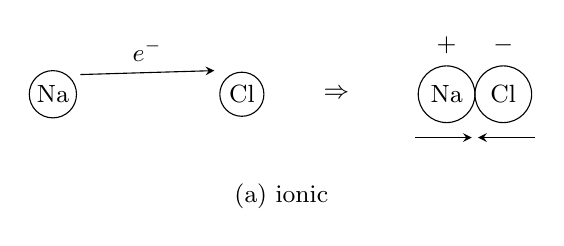
\begin{tikzpicture}[>=stealth, font=\small]
		\draw (0,0) circle (0.3) node {Na};
		\draw (2.4,0) circle (0.28) node {Cl};
		\draw[->] (0.35,0.25) -- (2.05,0.3);
		\node at (1.2,0.55) {$e^-$};
		\node at (3.6,0) {$\Rightarrow$};
		\draw (5.0,0) circle (0.36) node {Na};
		\draw (5.72,0) circle (0.36) node {Cl};
		\node at (5.0,0.62) {$+$};
		\node at (5.72,0.62) {$-$};
		\draw[->] (4.6,-0.55) -- (5.32,-0.55);
		\draw[->] (6.12,-0.55) -- (5.4,-0.55);
		\node at (2.9,-1.3) {(a) ionic};
	\end{tikzpicture}
	\hspace{1.5cm}
	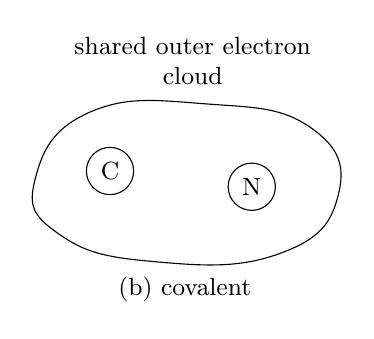
\begin{tikzpicture}[font=\small]
		\draw plot[smooth cycle, tension=0.8] coordinates {(-1.9,0.1) (-1.2,0.95) (0.3,1.05) (1.6,0.75) (1.95,-0.1) (1.2,-0.85) (-0.4,-0.95) (-1.6,-0.6)};
		\draw (-0.95,0.2) circle (0.3) node {C};
		\draw (0.85,0.0) circle (0.3) node {N};
		\node[align=center] at (0.1,1.6) {shared outer electron\\cloud};
		\node at (0,-1.3) {(b) covalent};
	\end{tikzpicture}
	\caption{(a) Ionic bonding: sodium gives an outer electron to chlorine, and the resulting ions attract each other. (b) Covalent bonding: the atoms share their outer electrons.}
	\label{f:bond}
\end{figure}
% NOTE: the caption and the panel labels (a), (b) are added; the two sketches are separate in the handwriting (page L7).

		% NOTE: "Energy states (cont.) - Different energy states" (page L8) continues the bullet "Let us consider each
		% energy state at a very high level" (page L7).
		\item[--] Different energy states
		\begin{itemize}
			\item Rotational energy
			\begin{itemize}
				% NOTE: added "(Figure~\ref{f:rot})".
				\item[$\hookrightarrow$] Our diatomic molecule can rotate ``end over end'' but can \underline{not} rotate about axis connecting atoms (Figure~\ref{f:rot}).

\begin{figure}[!htbp]
	\centering
	% Reproduces the handwritten sketch (page L8), element by element: a vertical axis with an arrowhead at the top
	% and a circular arrow around it (arrowhead on its right); an axis toward the lower right with an arrowhead and a
	% circular arrow around it (arrowhead at its top); the molecular axis (faint, thin line in the scan) through the
	% origin, joining two shaded atoms at the lower left and upper right; a small upward arrow pointing at the
	% molecular axis from the label "no rotation about this axis (can't rotate relative to one another and
	% synchronous rotation is meaningless -> virt. no energy)".
	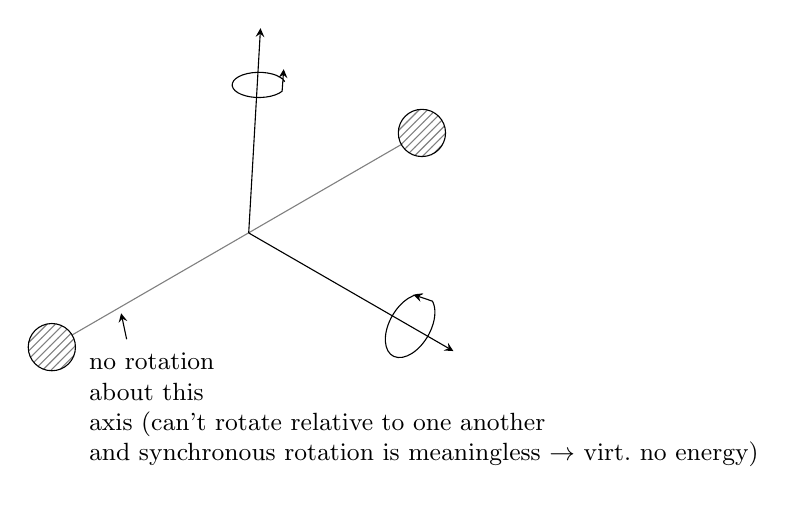
\begin{tikzpicture}[>=stealth, font=\small, scale=1.0]
		\coordinate (O) at (0,0);
		% molecular axis and atoms
		\draw[thin, gray] (-2.25,-1.3) -- (1.95,1.13);
		\draw[pattern=north east lines, pattern color=gray] (-2.5,-1.45) circle (0.3);
		\draw[pattern=north east lines, pattern color=gray] (2.2,1.27) circle (0.3);
		% vertical axis with circular arrow
		\draw[->] (O) -- (0.15,2.6);
		\draw[->] (0.13,1.88) ++(15:0.34 and 0.16) arc (15:330:0.34 and 0.16) -- ++(0.02,0.28);
		% lower-right axis with circular arrow
		\draw[->] (O) -- (2.6,-1.5);
		\begin{scope}[shift={(2.05,-1.18)}, rotate=60]
			\draw[->] (15:0.44 and 0.26) arc (15:340:0.44 and 0.26) -- ++(-0.05,0.25);
		\end{scope}
		% label and pointer to the molecular axis
		\draw[->] (-1.55,-1.35) -- (-1.62,-1.02);
		\node[anchor=north west, align=left] at (-2.15,-1.4) {no rotation\\about this\\axis (can't rotate relative to one another\\and synchronous rotation is meaningless $\rightarrow$ virt.\ no energy)};
	\end{tikzpicture}
	\caption{A diatomic molecule rotates ``end over end'' about the two axes perpendicular to the line joining the atoms, but not about that line.}
	\label{f:rot}
\end{figure}
% NOTE: the caption is added. "virt." (virtually) is a low-confidence reading of the handwriting.

				\item[$\hookrightarrow$] laws of quantum mechanics require rotations only at discrete rates or frequencies (not continuous as in classical mechanics)
				\item[$\hookrightarrow$] But like classical mechanics, higher rotation rates imply higher energy
				\item[$\hookrightarrow$] discrete rotation rates and rates $\leftrightarrow$ energy $\Rightarrow$ described by ``rotation levels'' $\rightarrow$ energy state $\mathcal{E}_\mathrm{r}$
				% NOTE: checked against Liou 2002, p. 18 (selection rule Delta J = +-1, with J the rotational quantum
				% number, written l here). The handwritten asterisks and underline are kept.
				\item[$\hookrightarrow$] Key feature is that rotational transitions can occur by absorbing or emitting photons, $*$\,\underline{but can only `jump' from one rotation level to another and only one at a time}\,$*$
				% NOTE: kept as handwritten; this is approximate (correspondence principle). The photon angular
				% frequency is the energy difference of the two levels divided by hbar, (hbar/I)(l + 1) for
				% l -> l + 1 with I the moment of inertia, which lies between the rotation rates of the lower and upper
				% levels, (hbar/I) sqrt(l(l+1)) and (hbar/I) sqrt((l+1)(l+2)) (from Liou 2002, Eqs. 1.3.5-1.3.6, p. 18;
				% python3 check).
				\item[$\hookrightarrow$] To move from one rotation level to another, molecule must absorb a photon with frequency equal to that of the next rotation level (frequency) $\Rightarrow$ to spin faster, molecules must absorb increasingly higher frequency EM radiation
				% NOTE: the handwritten "(conversely,)" is inserted with a caret.
				\item[$\hookrightarrow$] (conversely,) to slow down, a molecule must emit EM radiation with frequency equal to the rotation level
				% NOTE: handwritten reads "rotation levels are equally spaced in energy, and hence frequency, therefore
				% absorption lines are equally spaced in frequency but not wavelength"; corrected because the rotational
				% energy levels are not equally spaced: U_r = Bhc J(J+1) (Liou 2002, Eq. 1.3.6, p. 18; J = l here), so
				% the gaps between adjacent levels grow in equal steps, 2, 4, 6, ... (in units of Bhc), and the lines of
				% the allowed one-level transitions are equally spaced, by 2B in wavenumber (Liou p. 18 and Fig. 1.10a,
				% p. 19). Equivalently, from U_r below with omega = L/I proportional to sqrt(l(l+1)) (Liou p. 18,
				% L = I omega), U_r is proportional to l(l+1). The conclusion (lines equally spaced in frequency but not
				% in wavelength) is unchanged.
				\item[$\hookrightarrow$] rotation levels are not equally spaced in energy ($\mathcal{E}_\mathrm{r} \propto J(J+1)$), but the energy differences between adjacent levels increase in equal steps (${\propto}\,J+1$), and hence so do the frequencies of the allowed one-level transitions; therefore absorption lines are equally spaced in frequency but not wavelength (Figure~\ref{f:lines}).

\begin{figure}[!htbp]
	\centering
	% Reproduces the handwritten sketch (page L9), element by element: top, an omega axis with its arrowhead at the
	% left (omega increasing to the left; label omega at the left end; a small tick at the right end) and four
	% equally spaced vertical lines omega_4, omega_3, omega_2, omega_1 from left to right; bottom, a lambda axis with
	% its arrowhead at the right, labeled lambda = 2 pi c/omega, and four lines lambda_4, lambda_3, lambda_2, lambda_1
	% from left to right. The line positions are computed from the rigid-rotor line frequencies omega_n = n omega_1
	% (equally spaced), so lambda_n = lambda_1/n.
	\begin{tikzpicture}[>=stealth, font=\small]
		\def\s{1.9}   % spacing in omega
		\def\xo{9.0}  % position of omega_1
		% omega axis
		\draw[->] (\xo+0.35,0) -- (1.5,0);
		\draw (\xo+0.35,0) -- ++(0.08,0.12);
		\node[anchor=east] at (1.45,0) {$\omega$};
		\foreach \n in {1,...,4} {
			\pgfmathsetmacro{\x}{\xo-(\n-1)*\s}
			\draw (\x,0) -- (\x,1.5);
			\node[anchor=north] at (\x,-0.05) {$\omega_{\n}$};
		}
		% lambda axis: x = x0 + k/n
		\def\xl{2.0}\def\kk{7.0}
		\draw[->] (1.5,-2.2) -- (\xo+0.6,-2.2);
		\node[anchor=west] at (\xo+0.65,-2.2) {$\lambda = 2\pi\dfrac{c}{\omega}$};
		\foreach \n in {1,...,4} {
			\pgfmathsetmacro{\x}{\xl+\kk/\n}
			\draw (\x,-2.2) -- (\x,-0.9);
			\node[anchor=north] at (\x,-2.25) {$\lambda_{\n}$};
		}
	\end{tikzpicture}
	\caption{Pure rotational absorption lines are equally spaced in frequency (top) but not in wavelength (bottom). The line positions are drawn with $\omega_2 = 2\omega_1$, $\omega_3 = 3\omega_1$, $\omega_4 = 4\omega_1$, so $\lambda_2 = \lambda_1/2$, $\lambda_3 = \lambda_1/3$, $\lambda_4 = \lambda_1/4$.}
	\label{f:lines}
\end{figure}
% NOTE: the caption is added.

				% NOTE: checked against Liou 2002, p. 18 (kinetic energy of a rigid rotating dipole L omega/2, with
				% L = I omega and L = (h/2 pi)[J(J+1)]^(1/2), Eq. 1.3.5), with J written l as handwritten. The
				% definition of omega (not defined in the handwriting) is added: here omega is the angular velocity of
				% the molecule's rotation, not the angular frequency of the EM wave.
				\item[$\hookrightarrow$] $\mathcal{E}_\mathrm{r} = \omega_\mathrm{rot}\hbar\sqrt{J(J+1)}/2$, where $\hbar \equiv$ reduced Planck constant ($\hbar = h/2\pi$), $J \equiv$ nonnegative integer called the rotational quantum number, and $\omega_\mathrm{rot} \equiv$ angular velocity of the rotation.
			\end{itemize}
			\item[--] Vibrational energy $\mathcal{E}_\mathrm{v}$
			\begin{itemize}
				\item[$\hookrightarrow$] dipoles can be `smushed' together along the line joining the atoms
				% NOTE: added "(Figure~\ref{f:vib})".
				\item[$\hookrightarrow$] basic process (Figure~\ref{f:vib})

\begin{figure}[!htbp]
	\centering
	% Reproduces the handwritten sketch (page L9), element by element. 1): two shaded atoms joined by a line, - above
	% the left and + above the right; a wave labeled "EM radiation" to the right, with its arrowhead at its left end
	% pointing at the + atom; below the atoms a rightward arrow (under -) and a leftward arrow (under +); the text
	% "positive side of dipole is pushed by EM radiation and negative side is pulled, causing the atomic nuclei to
	% move closer to one another". 2): two shaded atoms joined by a spring; below, a leftward arrow (under the left
	% atom) and a rightward arrow (under the right atom); the text "nuclei are both positively charged => repel
	% (analogous to a spring connecting two weights)". A curved arrow with arrowheads at both ends, bowed downward,
	% links 1) and 2), above the text "=> EM radiation pushes nuclei together, like charges repel => vibration".
	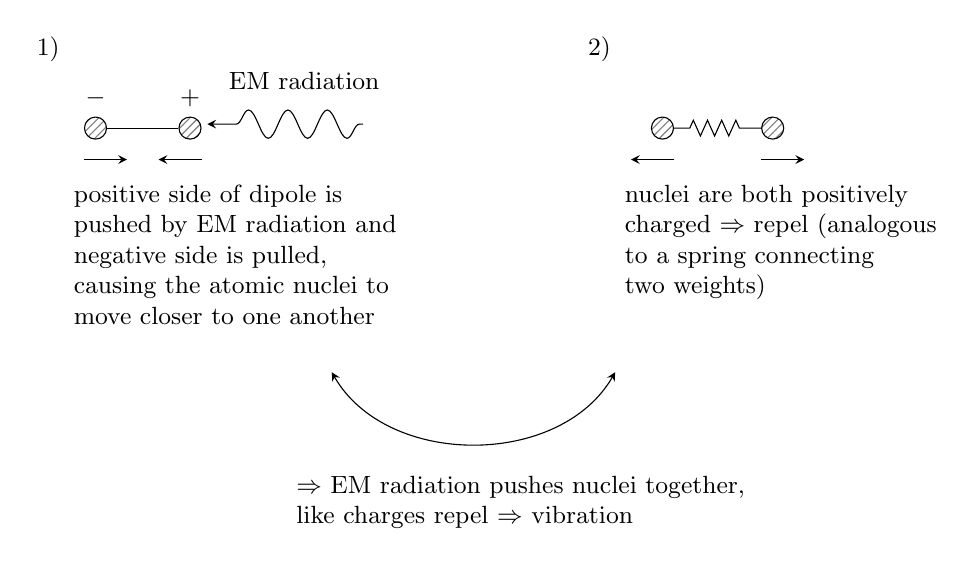
\begin{tikzpicture}[>=stealth, font=\small]
		\tikzset{atom/.style={draw, circle, minimum size=0.28cm, inner sep=0pt, pattern=north east lines, pattern color=gray}}
		% 1)
		\node at (-0.6,1.0) {1)};
		\node[atom] (a1) at (0,0) {};
		\node[atom] (b1) at (1.2,0) {};
		\draw (a1) -- (b1);
		\node at (0,0.38) {$-$};
		\node at (1.2,0.38) {$+$};
		\draw[->, decorate, decoration={snake, amplitude=0.18cm, segment length=0.5cm, pre length=0.05cm, post length=0.12cm}] (3.4,0.05) -- (1.42,0.05);
		\node at (2.65,0.6) {EM radiation};
		\draw[->] (-0.15,-0.4) -- (0.4,-0.4);
		\draw[->] (1.35,-0.4) -- (0.8,-0.4);
		\node[anchor=north west, align=left] at (-0.4,-0.6) {positive side of dipole is\\pushed by EM radiation and\\negative side is pulled,\\causing the atomic nuclei to\\move closer to one another};
		% 2)
		\node at (6.4,1.0) {2)};
		\node[atom] (a2) at (7.2,0) {};
		\node[atom] (b2) at (8.6,0) {};
		\draw[decorate, decoration={zigzag, amplitude=0.1cm, segment length=0.18cm, pre length=0.2cm, post length=0.2cm}] (a2) -- (b2);
		\draw[->] (7.35,-0.4) -- (6.8,-0.4);
		\draw[->] (8.45,-0.4) -- (9.0,-0.4);
		\node[anchor=north west, align=left] at (6.6,-0.6) {nuclei are both positively\\charged $\Rightarrow$ repel (analogous\\to a spring connecting\\two weights)};
		% link and conclusion
		\draw[<->] (3.0,-3.1) to[out=-60, in=-120] (6.6,-3.1);
		\node[align=left] at (5.4,-4.75) {$\Rightarrow$ EM radiation pushes nuclei together,\\like charges repel $\Rightarrow$ vibration};
	\end{tikzpicture}
	\caption{Basic process of molecular vibration driven by EM radiation.}
	\label{f:vib}
\end{figure}
% NOTE: the caption is added.

				\item[$\hookrightarrow$] frequency of vibrations are quantized $\rightarrow$ vibration levels
				\item[$\hookrightarrow$] When a molecule absorbs EM radiation of the frequency associated with a higher vibration level, a vibration transition occurs
				% NOTE: checked against U&L 2014, p. 329 ("vibrational transitions never occur alone, but are always
				% accompanied by many rotational transitions") and Liou 2002, p. 17. The one-level rule (Delta J = +-1)
				% holds for the diatomic molecules considered here; perpendicular vibrational modes of polyatomic
				% molecules (e.g., the CO2 bending mode) also allow Delta J = 0, the Q branch (Liou p. 20). The
				% handwritten asterisks and underline are kept. Added "(Figure~\ref{f:vibrot})".
				\item[$\hookrightarrow$] $*$\,However\,$*$ vibration transitions are always accompanied by a rotation transition $\rightarrow$ as we saw in the previous section, rotation transitions involve jumps of \underline{one and only one} level (can be up or down) (Figure~\ref{f:vibrot})

\begin{figure}[!htbp]
	\centering
	% Reproduces the handwritten sketch (page L10), element by element: a wave labeled "EM radiation" with its
	% arrowhead at the right end pointing at the lower-left shaded atom; a spring from that atom to the upper-right
	% shaded atom; a straight double-headed arrow parallel to the spring, below and to the right of it, labeled
	% "Vibration transition"; a curved arrow over the upper atom with its arrowhead at the left end, labeled
	% "rotation transition up or down by 1 level only".
	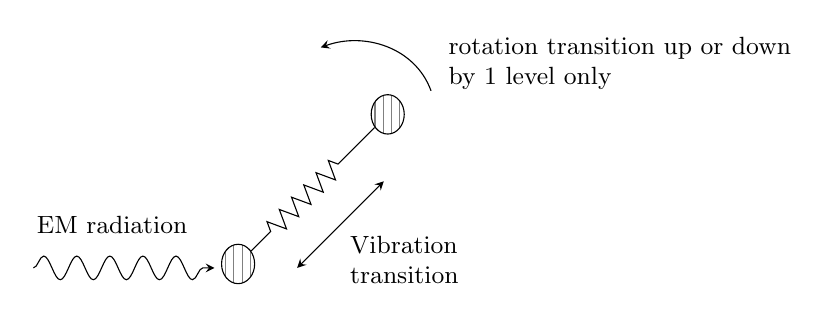
\begin{tikzpicture}[>=stealth, font=\small]
		\tikzset{atom/.style={draw, ellipse, minimum width=0.42cm, minimum height=0.5cm, inner sep=0pt, pattern=vertical lines, pattern color=gray}}
		\node[atom] (A) at (0,0) {};
		\node[atom] (B) at (1.9,1.9) {};
		\draw[decorate, decoration={zigzag, amplitude=0.12cm, segment length=0.22cm, pre length=0.35cm, post length=0.6cm}] (A) -- (B);
		\draw[->, decorate, decoration={snake, amplitude=0.15cm, segment length=0.42cm, post length=0.12cm}] (-2.6,-0.05) -- (-0.3,-0.05);
		\node at (-1.6,0.5) {EM radiation};
		\draw[<->] (0.75,-0.05) -- (1.85,1.05);
		\node[anchor=west, align=left] at (1.3,0.05) {Vibration\\transition};
		\draw[->] (2.45,2.2) to[out=110, in=20] (1.05,2.75);
		\node[anchor=west, align=left] at (2.55,2.55) {rotation transition up or down\\by 1 level only};
	\end{tikzpicture}
	\caption{A vibration transition driven by EM radiation, accompanied by a rotation transition of one level.}
	\label{f:vibrot}
\end{figure}
% NOTE: the caption is added.

				\item[$\hookrightarrow$] Since each vibration level can be associated with several rotation (sub-)levels, there are many possible vibration transitions within a population
				% NOTE: checked against Liou 2002, p. 20 and Fig. 1.10b (p. 19): the rotational level spacings are
				% smaller in the upper vibrational level, so the line spacing decreases toward higher wavenumber.
				\item[$\hookrightarrow$] All vibration transitions require slightly different energy levels, results in a series of closely spaced absorption lines that converge at short wavelengths (i.e., higher frequencies) $\Rightarrow$ absorption bands
				% NOTE: checked against U&L 2014, p. 329 (vibration-rotation bands "occur between the red part of the
				% visible spectrum and the thermal infrared region").
				\item[$\hookrightarrow$] Key point is that a range of higher frequency EM can be absorbed by molecules in the atmosphere $\rightarrow$ visible red to thermal infrared portion of EM spectrum
				% NOTE: checked against Liou 2002, Eq. 1.3.7 (p. 18), E_v = h nu_k (v_k + 1/2) with nu_k the frequency
				% of normal mode k (hbar omega = h nu). The definition of omega (not defined in the handwriting) is
				% added: here omega is the natural angular frequency of the vibration.
				\item[$\hookrightarrow$] $\mathcal{E}_\mathrm{v} = \left(n_\mathrm{vib} + \tfrac{1}{2}\right)\hbar\omega_\mathrm{vib}$, where $n_\mathrm{vib}$ is an integer called the vibrational quantum number (and $\omega_\mathrm{vib}$ is the natural angular frequency of the vibration).
			\end{itemize}
		\end{itemize}
	\end{itemize}
\end{itemize}

%%%%%%%%%%%%%%%%%%%%%%%%%%%%%%%%%%%%%
% Symbols follow the master table in ../variables_master.tex; see it for flagged dual usages.
\clearpage
\section*{Variables}

Units are SI. Values are given for universal constants; ``typical'' values are representative, not definitive.

{\small
\renewcommand{\arraystretch}{1.2}
\begin{longtable}{>{$}l<{$} >{\raggedright\arraybackslash}p{0.40\textwidth} >{\raggedright\arraybackslash}p{0.13\textwidth} >{\raggedright\arraybackslash}p{0.22\textwidth}}
\hline
\textrm{Symbol} & Description & Units & Value \\
\hline
\endfirsthead
\hline
\textrm{Symbol} & Description & Units & Value \\
\hline
\endhead
\hline
\endfoot
\multicolumn{4}{l}{\emph{Constants}} \\
c & speed of light in a vacuum & m/s & $2.998\times10^{8}$ \\
g & gravitational acceleration & m/s$^2$ & $9.81$ \\
R_\mathrm{gas} & universal gas constant & J\,mol$^{-1}$K$^{-1}$ & $8.314$ \\
h & Planck constant & J\,s & $6.626\times10^{-34}$ \\
\hbar & reduced Planck constant, $h/2\pi$ & J\,s & $1.055\times10^{-34}$ \\
\multicolumn{4}{l}{\emph{Atmosphere}} \\
z & altitude (height above sea level) & m & -- \\
T & temperature & K & -- \\
T_0 & sea-level standard temperature & K & $288.15$ \\
P & pressure & Pa & -- \\
P_0 & sea-level pressure & Pa & $1.013\times10^{5}$ ($1013.25$ mbar) \\
\rho_\mathrm{air} & mass density of dry air & kg/m$^3$ & -- \\
\rho_{\mathrm{air},0} & density of dry air at sea level & kg/m$^3$ & $1.225$ \\
c_p & specific heat of dry air at constant pressure & J\,kg$^{-1}$K$^{-1}$ & ${\sim}10^3$ (1004) \\
M & molar mass of dry air & kg/mol & $2.9\times10^{-2}$ \\
a & temperature lapse rate, $-dT/dz$ & K/m & $6.5$ K/km (standard atmosphere) \\
a_\mathrm{d} & dry adiabatic lapse rate, $g/c_p$ & K/m & ${\approx}9.8$ K/km \\
a_\mathrm{moist} & moist adiabatic lapse rate & K/m & -- \\
H_p & pressure scale height, $R_\mathrm{gas}T_0/(gM)$ & m & ${\approx}8.4$ km \\
H_\rho & density scale height & m & ${\approx}H_p$ \\
\rho_\mathrm{vap} & water-vapor density & kg/m$^3$ & -- \\
\rho_{\mathrm{vap},0} & water-vapor density at sea level (standard atmosphere) & kg/m$^3$ & $7.72\times10^{-3}$ \\
H_\mathrm{vap} & water-vapor scale height & m & 2--2.5 km \\
\multicolumn{4}{l}{\emph{Molecular energy states}} \\
\mathcal{E} & total internal energy of a molecule & J & $\mathcal{E}_\mathrm{e}+\mathcal{E}_\mathrm{v}+\mathcal{E}_\mathrm{r}$ \\
\mathcal{E}_\mathrm{e},\ \mathcal{E}_\mathrm{v},\ \mathcal{E}_\mathrm{r} & electronic, vibrational and rotational energy & J & -- \\
e^- & electron & -- & -- \\
J & rotational quantum number & dimensionless & $0, 1, 2, \ldots$ \\
n_\mathrm{vib} & vibrational quantum number & dimensionless & $0, 1, 2, \ldots$ \\
\omega & angular frequency of the EM radiation (Figure~\ref{f:lines}) & rad/s & -- \\
\omega_\mathrm{rot} & angular velocity of a molecule's rotation & rad/s & -- \\
\omega_\mathrm{vib} & natural angular frequency of a molecular vibration & rad/s & -- \\
\omega_1, \ldots, \omega_4 & angular frequencies of rotational absorption lines 1--4 & rad/s & $\omega_2 = 2\omega_1$, etc.\ (rigid rotor) \\
\lambda;\ \lambda_1, \ldots, \lambda_4 & wavelength; wavelengths of lines 1--4 & m & $2\pi c/\omega$ \\
\end{longtable}
}

\end{document}
